%!TEX root = volumeFinal.tex 

\chapter{\label{chap:proj}Projeto de Implementação}

Este capítulo apresenta o jogo MicroRTS, que foi escolhido para ser utilizado como plataforma para a implementação do algoritmo de AHTN. Este capítulo também apresenta como funciona o planejador HTN, que será utilizado para a geração de planos.

\section{MicroRTS}  \label{sec:microrts}

Jogos eletrônicos são muito populares, principalmente pela grande quantidade de gêneros, existem jogos de ação, aventura, esportes, estratégia, entre outros. Hoje em dia, os jogos buscam que quem jogue consiga ficar imerso no dentro do jogo, sem conseguir identificar um padrão nos jogadores fictícios, pois se não o jogo deixa de ser tão interessante. Para que isso aconteça, a IA é associada a diversos jogos, e é comum pensar que quanto mais complexa a IA aplicada dentro do jogo mais difícil jogo irá ficar, mas isso nem sempre é verdade. Não é sempre que uma IA complicada terá melhor desempenho do que uma mais simples. Uma boa IA, para jogos, é feita a partir do comportamento desejado para o jogo com os algoritmo certos~\cite{millington2009artificial}.

Jogos de estratégia em tempo real, também conhecidos por \textit{real-time strategy games} (RTS), é um subgênero de jogos de estratégia. 
Nesse gênero de jogo os jogadores devem construir uma base, buscar recursos, construir edificações, treinar unidades de ataques e aprimorar suas tecnologias.
O objetivo final do jogo é destruir uma ou mais bases inimigas. 
Alguns fatores que dificultam o desenvolvimento de IAs para jogos RTS. 
Os fatores estão relacionados com a complexidade dos jogos, pois os jogos RTS possuem um grande espaço de estados.
Além disso os jogadores realizam as jogadas ao mesmo tempo, fazendo com que cada jogador tenha um curto espaço de tempo para realizar as suas ações.
Por essa razão, não é possível traduzir automaticamente as técnicas de IA para jogos RTS sem algum tipo de abstração ou simplificação~\cite{ontanon2013survey, buro2012real}.

Um exemplo deste gênero é o MicroRTS\footnote{https://github.com/santiontanon/microrts}, uma simplificação de jogos como Starcraft\footnote{http://us.battle.net/sc2/pt/}. 
O MicroRTS foi desenvolvido por Santiago Ontañón~\cite{ontanon2013combinatorial} em Java para fins acadêmicos, com o intuito de aplicar e desenvolver técnicas de IA e para servir como prova de conceito para as técnicas criadas.
O MicroRTS consiste em dois jogadores tentando destruir a base adversaria. 
Para ganhar o jogo é preciso eliminar cada unidade e edificação do adversário. 
O jogo termina quando um dos dois jogadores não tem mais unidades, ou quando o jogo atinge o limite de tempo. 
A Figura~\ref{fig:microrts} mostra um exemplo de tela do jogo.

\begin{figure}[ht]
	\centering
	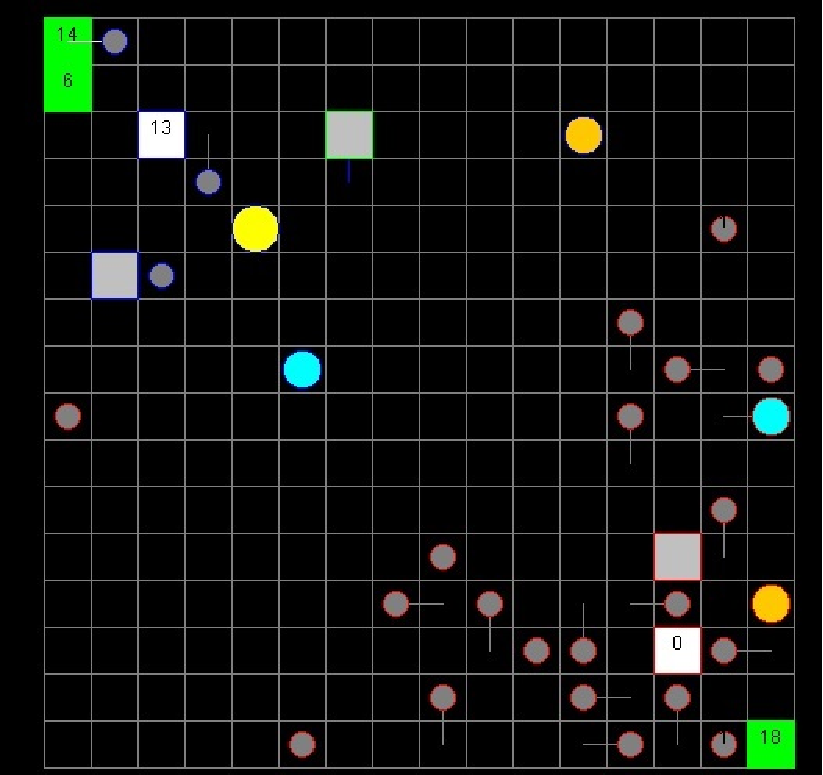
\includegraphics[width=0.5\textwidth]{fig/microrts.pdf}
	\caption{Um exemplo de tela do MicroRTS}
	\label{fig:microrts}
\end{figure} 

\subsection{Unidades e construções}
No MicroRTS existem quatro tipos de unidades no jogo, e cada uma foi descrita a seguir:

\begin{itemize}
	\item \textit{worker}, é responsável por coletar recursos e construir as edificações. Esta unidade também consegue lutar, mas possui um dano muito baixo;
	\item \textit{heavy}, unidade que pode apenas atacar. Ela possui um alto poder de ataque, mas sua velocidade é lenta;
	\item \textit{light}, unidade que pode apenas atacar. Ela possui um baixo poder de ataque, mas sua velocidade é rápida; e
	\item \textit{ranged}, unidade que pode apenas atacar. Ela possui um ataque de longa distância. 
\end{itemize} 

Para treinar as unidades é preciso ter recursos e edificações. 
No MicroRTS é preciso ter uma base que é a edificação principal. 
A base é responsável pela criação dos \textit{workers}.
Ela também é responsável pelo armazenamento dos recursos, que são necessários para treinar e construir tudo dentro do jogo. 
O quartel é responsável pela criação das unidades de ataque que podem apenas atacar. 
Ela pode ser construída apenas por \textit{workers} e é preciso utilizar uma quantidade de recurso para a sua construção. 
Os recursos são obtidos através dos \textit{workers}, que extraem recursos da base de recurso e armazenam na base. 

\subsection{Arquitetura}

O MicroRTS conta com cinco classes principais para funcionamento do jogo. 
Cada classe é responsável por um controle dentro do jogo.
As classes \textit{GameState} e \textit{PhysicalGameState} são responsáveis pelo controle das ações das unidades dentro do mapa.
A \textit{UnitTypeTable} é utilizada para associar cada unidade com as suas ações possíveis.
A classe \textit{PhysicalGameStatePanel} é responsável pela interface gráfica.
A classe \textit{GameVisualSimulation} é utilizada para unir todos os componentes do jogo, e configurar as informações de mapa, jogadores, humanos ou IAs, e tempo de duração da partida.
O diagrama de classes presente na Figura~\ref{fig:classes} ilustra como as classes se relacionam e seus principais métodos.

\begin{figure}[ht]
	\centering
	\frm[inline]{Nope, I want vector graphics, man! And text of a size that I can read.}
	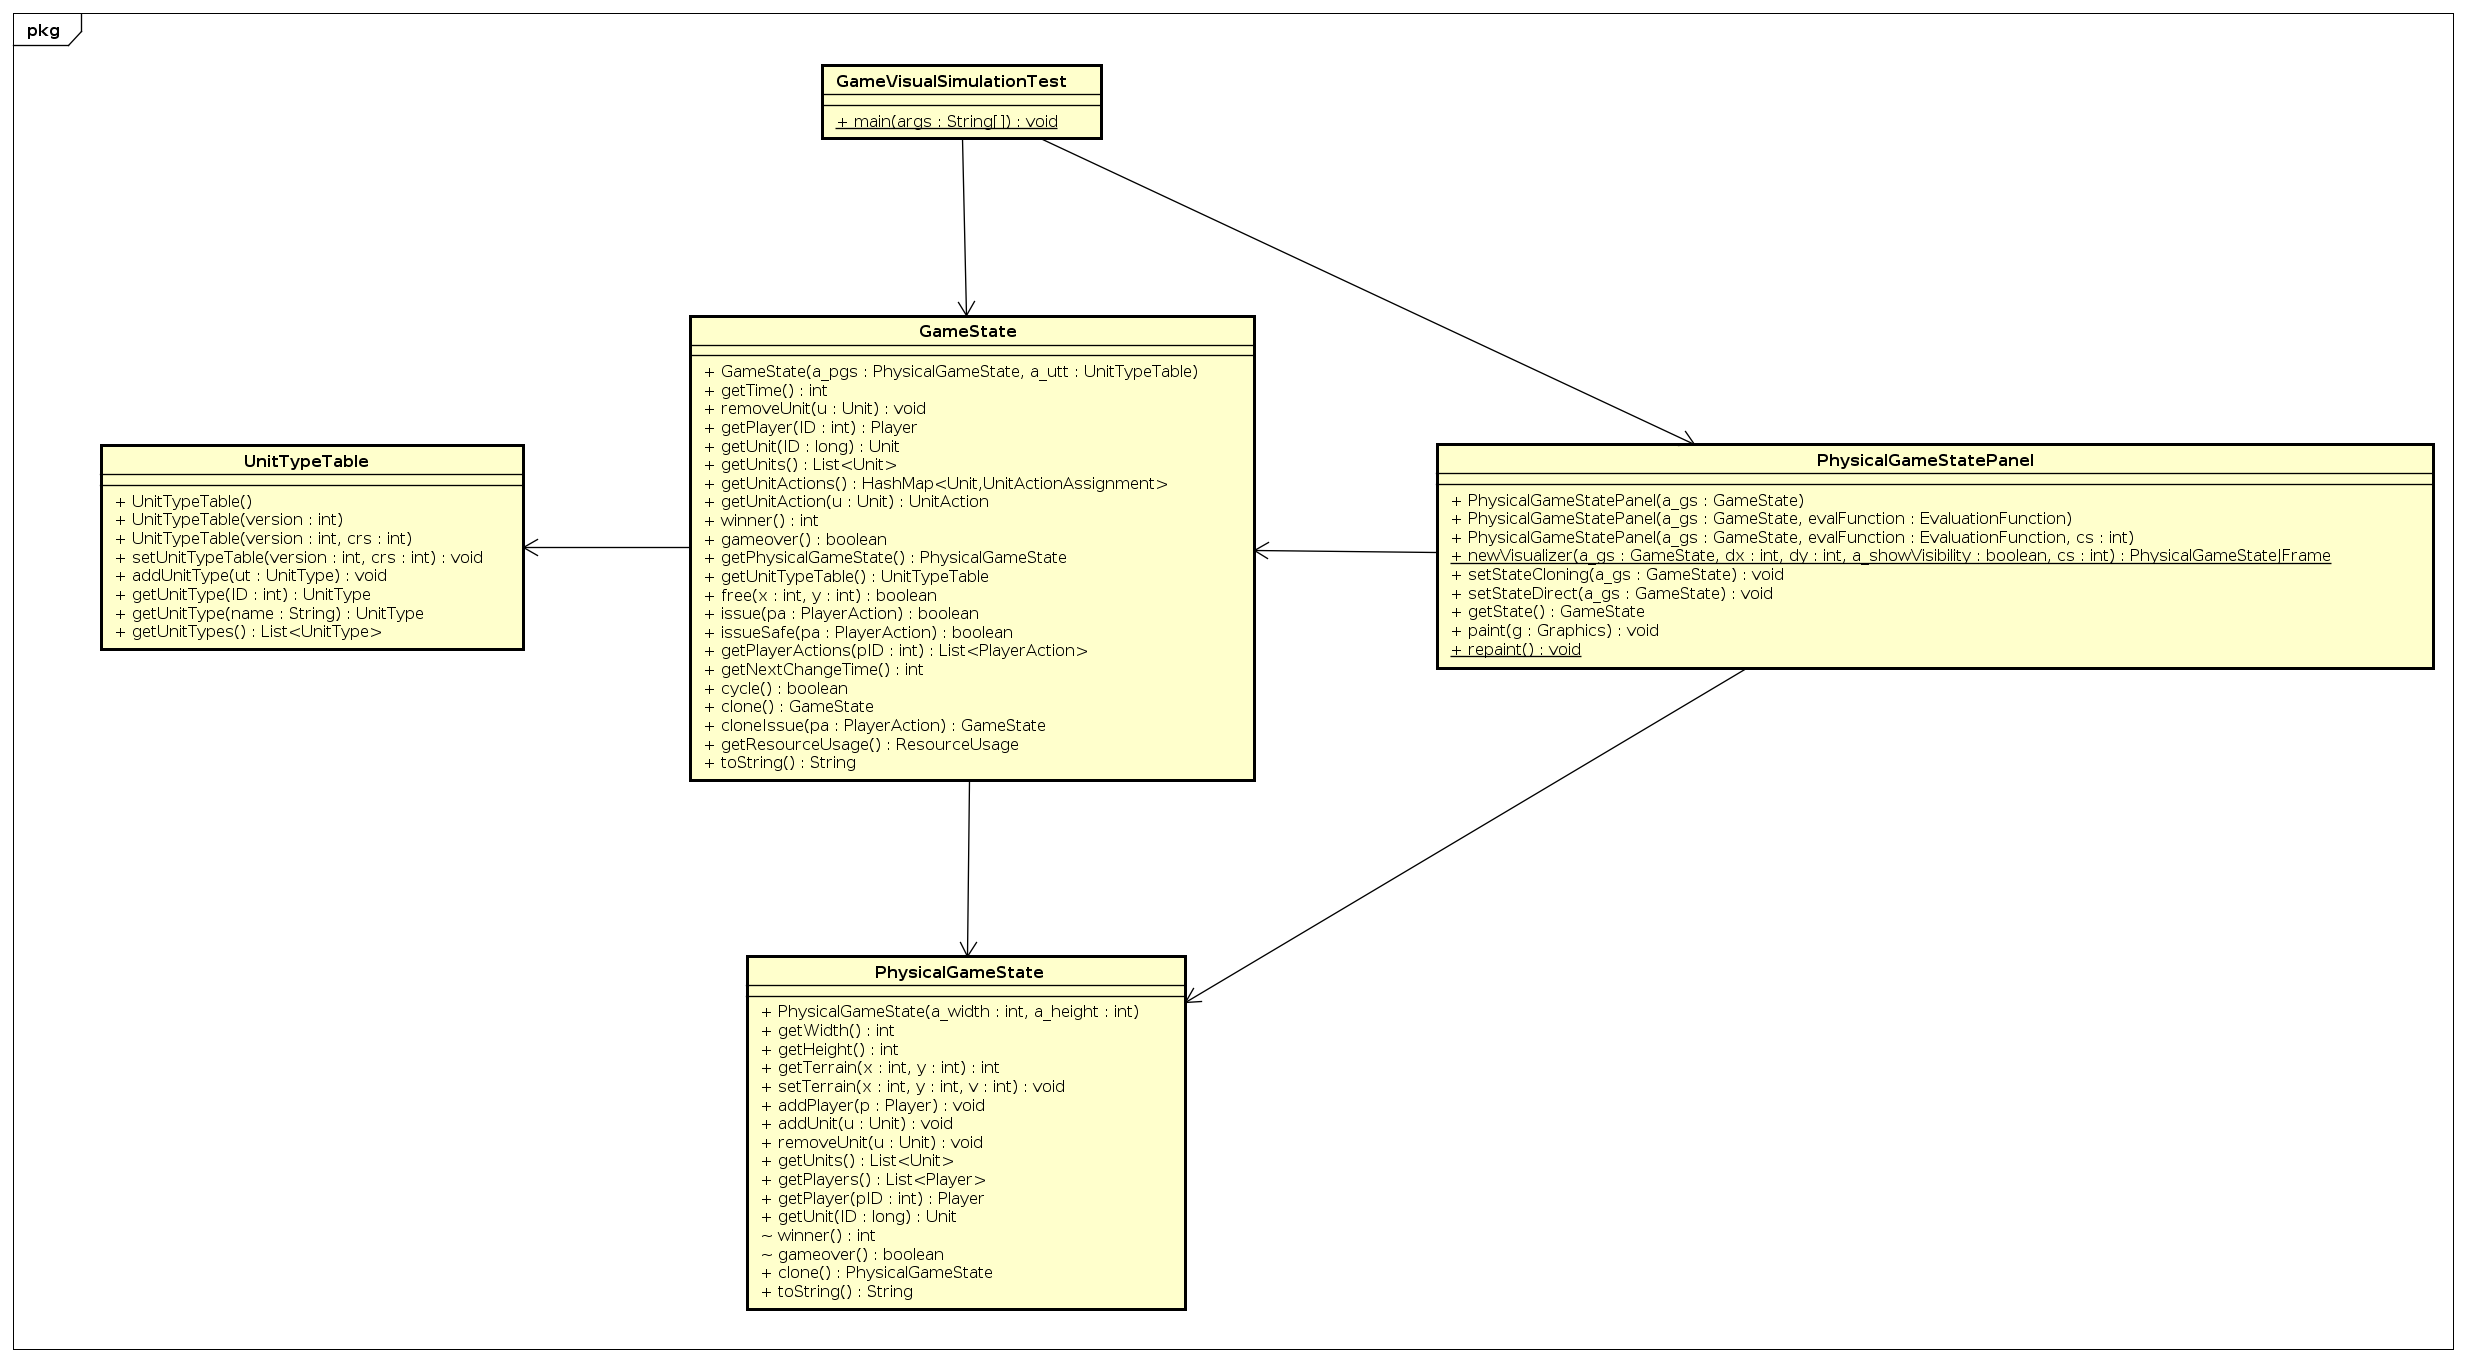
\includegraphics[width=1\textwidth]{fig/classes.png}
	\caption{Classes do MicroRTS}
	\label{fig:classes}
\end{figure} 

O MicroRTS fornece uma camada de abstração para que se possa utilizar as unidades, sem precisar ter conhecimento de como elas estão estruturadas. 
Essa camada se chama \textit{AbstractionLayerAI}. 
Ela apresenta métodos para treinar unidades, construir edificações, coletar recursos, atacar, e movimentar as unidades. 
Esta camada oferece todos os recursos necessários para que seja implementado uma IA.

Toda a IA que for implementada no MicroRTS deve conter o método $\mathit{getAction}$.
Este método é responsável por determinar qual ação deve ser realizada pela IA em determinado momento do jogo.
Cada IA pode assumir o lugar de um jogador no MicroRTS. 
A classe \textit{GameVisualSimulation}, que é responsável por gerenciar a simulação, inicializa os jogadores e a cada período de tempo chama o método realizar as ações dos jogadores.
A Figura~\ref{fig:sequencia} ilustra o diagrama de sequência do funcionamento da classe \textit{GameVisualSimulation}. 

\todo[inline]{Felipe, pode ler daqui em diante. Obrigado}

O algoritmo Algoritmo~\ref{alg:jogo} apresenta o pseudo código da classe. 
A classe primeiro obtém as instâncias dos objetos necessários para a simulação do jogo, esse processo está representado a partir da linha~\ref{alg:jogo:instancia} até a linha~\ref{alg:jogo:instanciaend}.
A linha~\ref{alg:jogo:desenha} é onde o algoritmo chama a classe da interface gráfica para desenhar a tela do jogo.
Após isso, o jogo entra em um laço para que os jogadores façam suas jogadas. As linhas~\ref{alg:jogo:action1} e \ref{alg:jogo:action2} são onde os jogadores escolhem qual as suas jogadas.
Nas linhas~\ref{alg:jogo:issue1} e \ref{alg:jogo:issue2} as jogadas são testadas para que não haja nenhuma violação quanto as restrições do jogo.
Na linha~\ref{alg:jogo:gameover} é responsável por determinar se o jogo não acabou.
A linha~\ref{alg:jogo:repaint} desenha a tela novamente com as jogadas executadas.
Assim o laço da linha~\ref{alg:jogo:while} é executado até que o jogo termine com algum vencedor, ou quando o tempo de simulação acabar.

\begin{algorithm}
	\caption{Pseudo código da classe \textit{GameVisualSimulation}.}
	\label{alg:jogo}
	\begin{algorithmic}[1]		
		\Function {main}{$String[]$}
		\State $utt = UnitTypeTable()$ \label{alg:jogo:instancia}
		\State $pgs = PhysicalGameState()$
		\State $gs = GameState(pgs, utt)$
		\State $player1 = Player1()$
		\State $player2 = Player2()$ \label{alg:jogo:instanciaend}
		\State $drawScreen()$  \label{alg:jogo:desenha}
		\While{$!gameover() || endTime()$} \label{alg:jogo:while}
			\State $action1 = player1.getAction()$ \label{alg:jogo:action1}
			\State $action2 = player2.getAction()$ \label{alg:jogo:action2}
			\State $issueSafe(action1)$ \label{alg:jogo:issue1}
			\State $issueSafe(action2)$ \label{alg:jogo:issue2}
			\State $gameover = gs.cycle()$ \label{alg:jogo:gameover} 
			\State $repaintScreen()$ \label{alg:jogo:repaint}
		\EndWhile
		\EndFunction
	\end{algorithmic}
\end{algorithm}

\begin{figure}[ht]
	\centering
	\frm[inline]{Está em PDF, mas ainda não é vetorial.}
	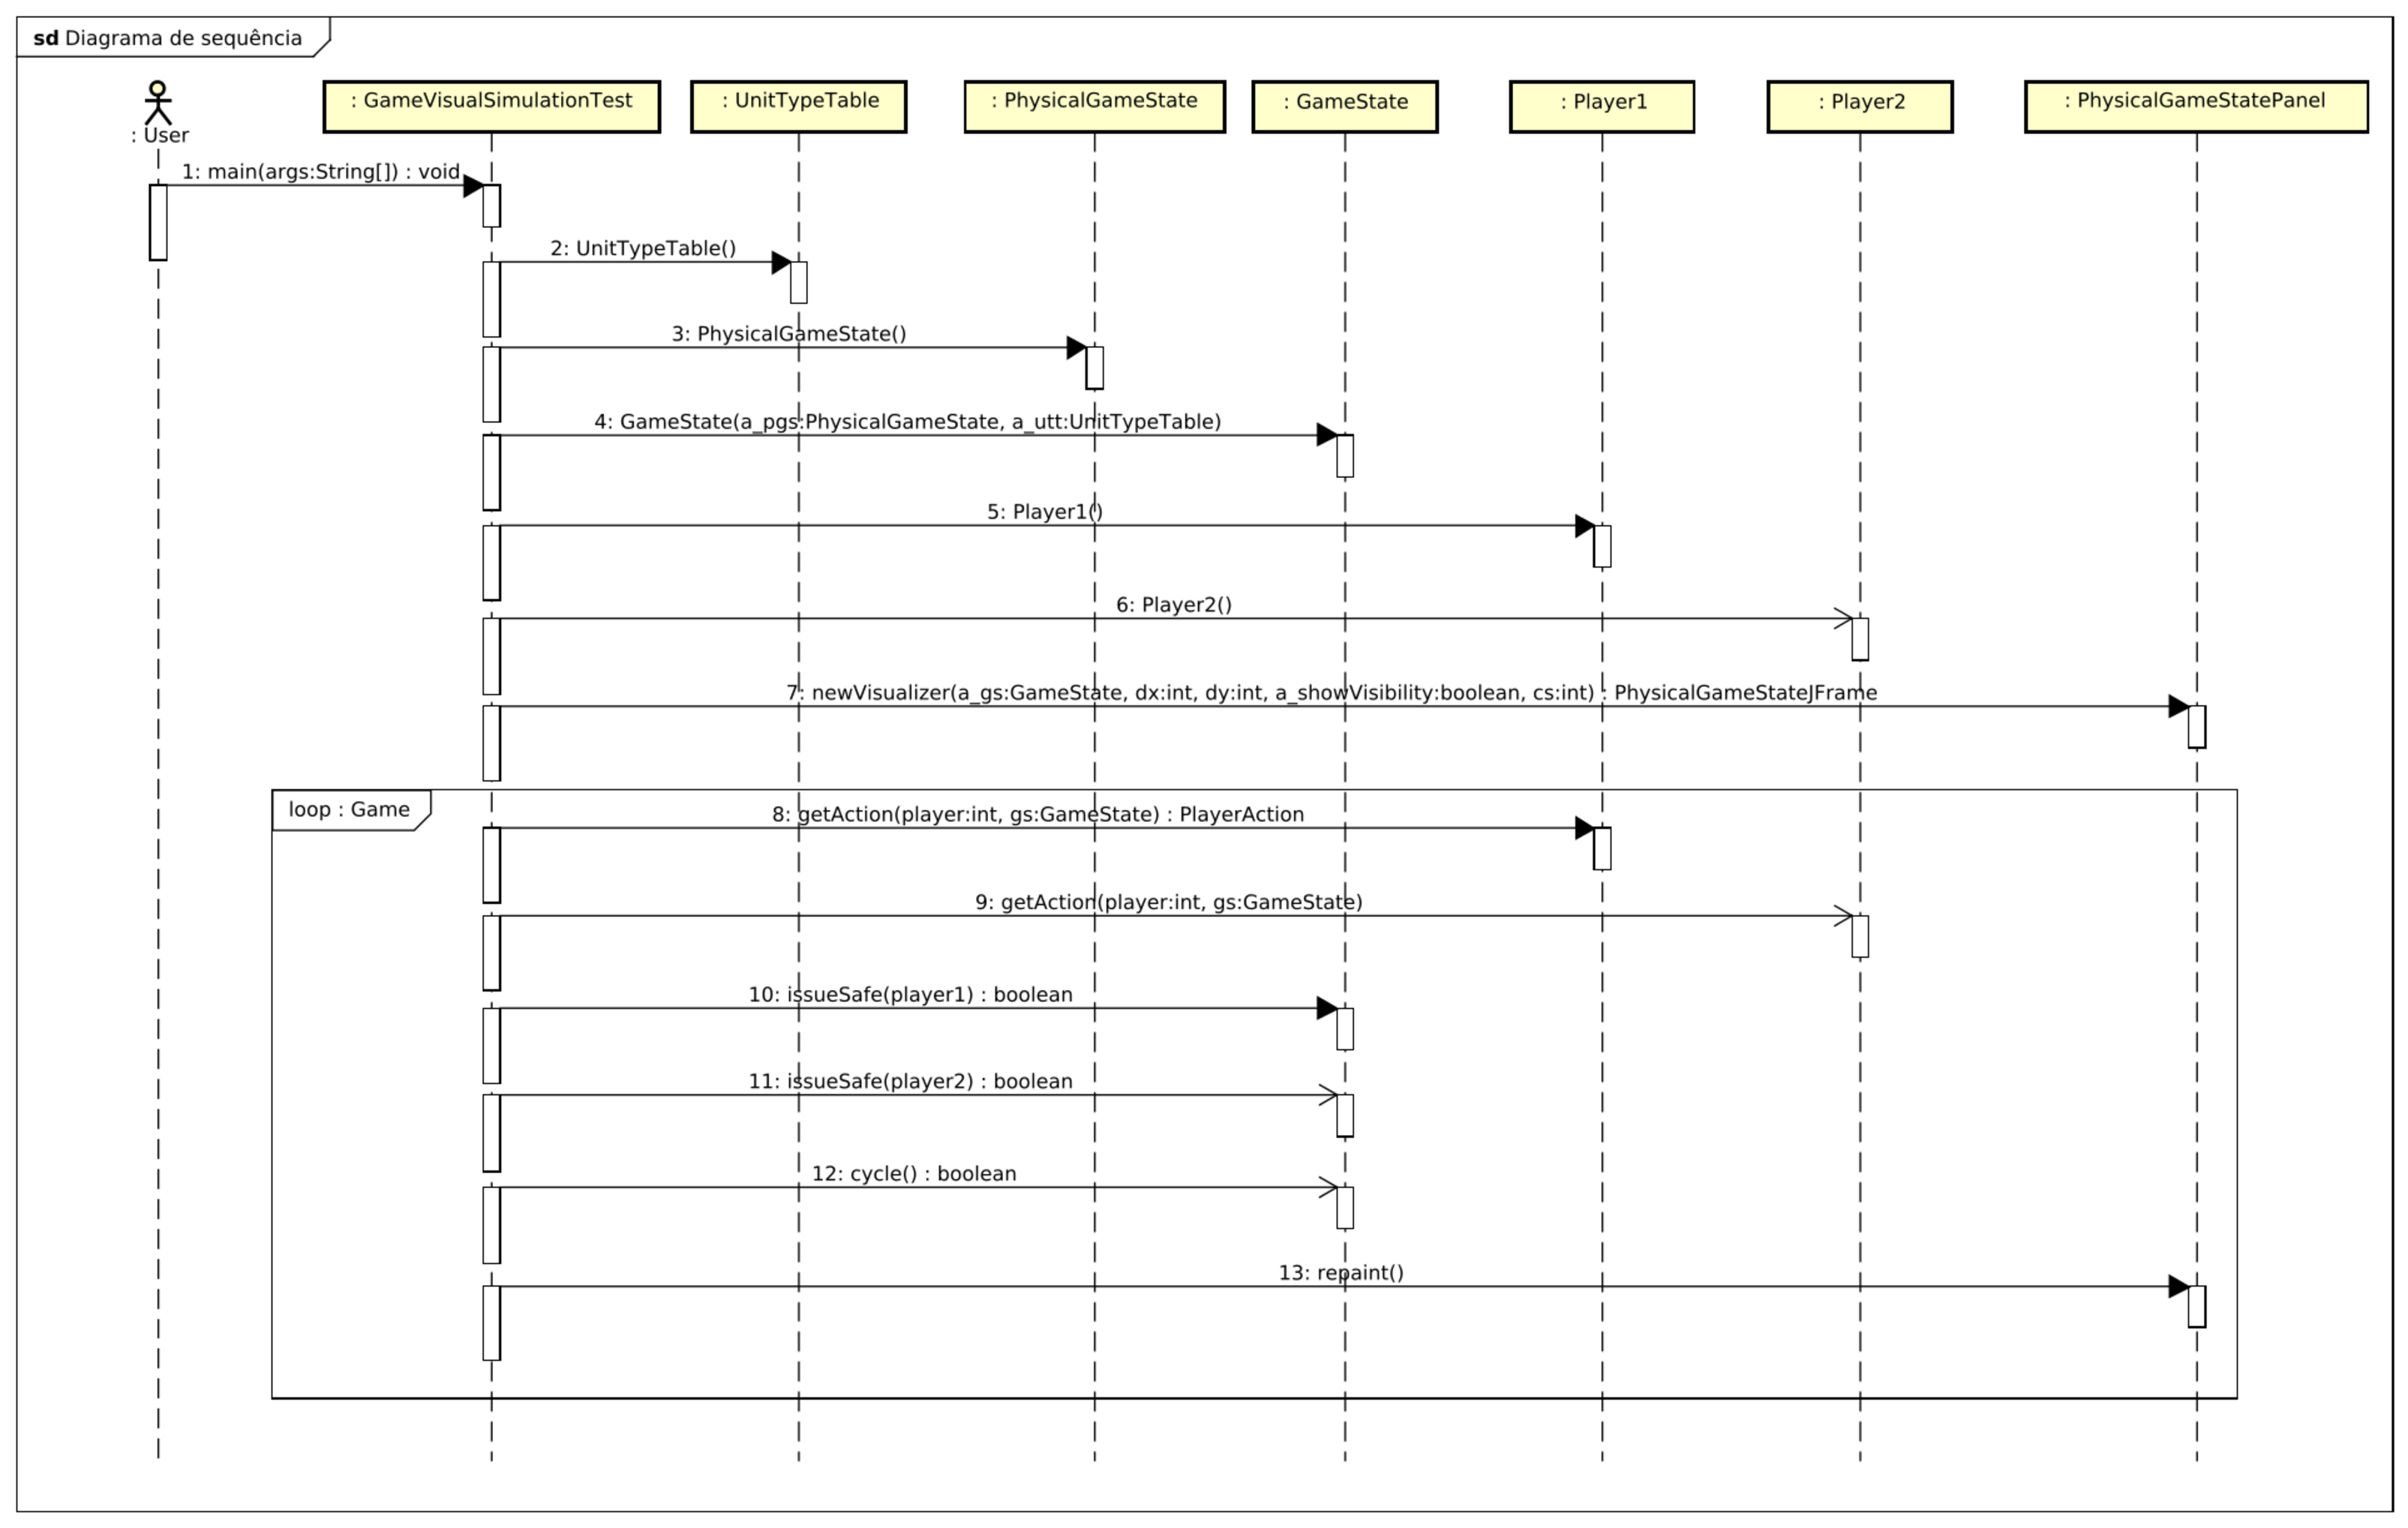
\includegraphics[width=1\textwidth]{fig/diagramaSequencia.pdf}
	\caption{Diagrama de sequência}
	\label{fig:sequencia}
\end{figure}

\subsection{Técnicas de IA} \label{sec:tecn}

O MicroRTS possui algumas técnicas de IA já implementadas.
Algumas destas técnicas simulam algum comportamento dentro do jogo, sem ter um algoritmo de IA, essas técnicas são chamadas de estratégias Hard-Coded. 
Dentro das estratégias Hard-Coded, existem duas técnicas que são baseadas em executar movimentos aleatórios, elas são chamadas de RandomAI e RandomBiasedAI.
A RandomAI executa movimentos totalmente aleatórios.
Já a RandomBiasedAI executa movimentos aleatórios mas com probabilidade maior de realizar movimentos de ataque, ou extração de recurso, ou criação de tropas.
Ainda dentre as estratégias Hard-Coded, existem técnicas que utilizam uma mesma dinâmica. 
Elas utilizam um \textit{worker} para extrair recursos, e treinam unidades de ataque para atacar. 
Essas técnicas se diferenciam no tipo de unidade de ataque que é criado. 
As técnicas são chamadas de LightRush, HeavyRush, e RangedRush, elas utilizam as unidades \textit{light}, \textit{heavy}, e \text{ranged}, respectivamente.
A ultima técnica deste tipo de categoria é chamada de WorkerRush, ela consiste ter um \textit{worker} para realizar a extração de recursos, mas ao invés de treinar unidades de ataque, ela treina outros \textit{workers} para realizar os ataques, isso faz com que a técnica consiga criar muitas unidades de maneira rápida.

Outras técnicas utilizam algum algoritmo de IA para decidir qual ação deve ser realizada.
Como é o caso das estratégias Minimax, Monte Carlo, e Portfolio Search.
A estratégia de Minimax utiliza o algoritmo de minimax para uma determinada profundidade. A profundidade não é em relação aos turnos, como no algoritmo comum de minimax, mas sim ao tempo disponível para tomar um decisão.
A estratégia de Monte Carlo verifica todas as ações possíveis para o estado, e simula jogos aleatórios para aquela jogada até um determinado tempo. Uma heurística é utilizada para determinar qual foi a ação que obteve o melhor valor.
Já estratégia de Portfolio Search possui um conjunto de estratégia e utiliza um algoritmo de busca para decidir qual a melhor estratégia para ser usada em determinado momento. O conjunto é composto pelas estratégias Hard-Coded.

\section{Java Simple Hierarchical Ordered Planner 2}\label{sec:jshop}
		
Java Simple Hierarchical Ordered Planner 2 (JSHOP2)~\cite{ilghami2006documentation} é um sistema de planejamento independente de domínio baseado em HTN. O JSHOP2 foi desenvolvido em Java por Dana Nau e sua equipe de pesquisa. 

O JSHOP2 recebe como entrada uma descrição do domínio e um problema de planejamento. 
A descrição do domínio contém a formalização das ações dos agentes, as tarefas e métodos que as decompõem.
O planejador realiza a geração do plano decompondo os métodos até que só restem tarefas primitivas. Na descrição do domínio as tarefas primitivas são descrita como operadores. Na descrição do domínio os operadores são compostos por um nome de operador, uma lista de precondições que deve ser verdadeira para a execução do operador, uma lista de elementos que serão removidos do estado, e uma lista de elementos que serão adicionados ao estado, um exemplo de operador é apresentado a seguir:

\lstset{style=codeStyle}
\begin{lstlisting}[language=lisp]
	(:operator (!move ?from ?to) 
		((at ?from)) 
		((at ?from))
		((at ?to))
	)
\end{lstlisting}

Os métodos são utilizados para decompor tarefas de alto nível para níveis mais baixos. No JSHOP2 os métodos são identificados por um nome de método, que é único para cada método. Dentro de um método há uma lista de precondições, e uma lista de tarefas, que podem ser primitivas ou não primitivas, para quantos casos forem necessário. Por exemplo, o problema de ir de um local para outro, se o local destino tem um caminho para o local origem, é possível se locomover para o local, mas se não houver caminho é preciso ir para outra cidade que tenha caminho para o local destino. Este exemplo pode ser visto abaixo:

\lstset{style=codeStyle}
\begin{lstlisting}[language=lisp]
	(:method (travel ?from ?to)
		((at ?from) (path ?from ?to))
		((!move ?from ?to))
		
		((not (path ?from ?to)) (path ?from ?somewhere))
		((!move ?from ?somewhere) (travel ?somewhere ?to))
	)
\end{lstlisting}

O domínio completo começa com o nome do domínio e em seguida os operadores e métodos descritos. O domínio completo exemplo ficaria assim: 

\lstset{style=codeStyle}
\begin{lstlisting}[language=lisp]
(defdomain move
	(
		(:operator (!move ?from ?to) 
			((at ?from)) 
			((at ?from))
			((at ?to))
		)
	
		(:method (travel ?from ?to)
			((at ?from) (path ?from ?to))
			((!move ?from ?to))
		
			((not (path ?from ?to)) (path ?from ?somewhere))
			((!move ?from ?somewhere) (travel ?somewhere ?to))
		)    
	)
)
\end{lstlisting}

O problema de planejamento contém as informações do estado do ambiente e qual é o objetivo do agente. 
O estado do ambiente é composto por predicados que são usados nos métodos e operadores, como no exemplo $at ?x$ e $path ?a ?b$. E o objetivo do agente é um método do domínio, no exemplo $travel ?from ?to$. Um possível problema de planejamento para o exemplo pode ser o apresentado abaixo:


\begin{lstlisting}[language=lisp]
(defproblem problem move
	( 
		(path PortoAlegre Charqueadas)
		(path Charqueadas SaoJeronimo)
		(at PortoAlegre)
	)
	
	(
		(travel PortoAlegre SaoJeronimo)
	)
)
\end{lstlisting}

O JSHOP2 gera duas classes java, uma representando o domínio, e a outra representando o problema.
A classe do problema gera o plano, utilizando as informações da classe da descrição do domínio.
Uma vez que o domínio esteja consolidado não é preciso gerar a classe do domínio novamente. A classe do problema deve mudar dependendo do estado do ambiente.  
O plano gerado para o exemplo acima é o seguinte:

\begin{lstlisting}[language=lisp]
[Plan cost: 2.0

(!move portoalegre charqueadas)
(!move charqueadas saojeronimo)
--------------------
]
\end{lstlisting}

O plano indica o custo do plano, junto com os operadores em ordem que devem ser executados para que o objetivo seja alcançado. 
Caso existam mais planos que levem ao mesmo objetivo, o JSHOP2 apresenta os planos na mesma estrutura.

Este capítulo apresenta todos os requisitos necessários para a implementação do algoritmo de AHTN.
A Seção~\ref{sec:microrts} apresenta como é o funcionamento do MicroRTS, e em qual parte do jogo o algoritmo pode ser implementado.
Na Seção~\ref{sec:jshop} é apresentado o planejador HTN que será utilizado para gerar os planos usados no algoritmo. 
No próximo capítulo é apresentado como foi feita a modelagem do domínio, a implementação do algoritmo de AHTN no MicroRTS, e como foi feita a tradução do cenário do jogo para um problema de planejamento.

